\documentclass[11pt,a4paper]{article}


\usepackage[utf8]{inputenc}
\usepackage[T1]{fontenc}
\usepackage[spanish,es-noquoting]{babel}
\usepackage[a4paper,margin=2.4cm]{geometry}
\usepackage{graphicx}
\usepackage{amsmath,amssymb}
\usepackage{booktabs}
\usepackage{array}
\usepackage{multirow}
\usepackage{siunitx}
\usepackage{caption}
\usepackage{subcaption}
\usepackage[hidelinks]{hyperref}
\usepackage{cite}
\usepackage{xcolor}
\usepackage{enumitem}
\usepackage{float}

\graphicspath{{figuras/}}

\captionsetup{font=small,labelfont=bf}
\setlength{\parskip}{0.35em}

% Caja placeholder para figuras aun no generadas.
% Reemplazar cada \figplaceholder por \includegraphics cuando exista la imagen.
\newcommand{\figplaceholder}[2][0.6\linewidth]{%
  \fbox{\parbox[c][#2][c]{#1}{\centering\small\textit{[Figura pendiente: reemplazar por imagen]}}}%
}

% Marca un espacio de contenido a completar (p. ej. por el companero).
\newcommand{\pendiente}[1]{%
  \par\medskip\noindent
  \fbox{\parbox{\dimexpr\linewidth-2\fboxsep-2\fboxrule}{%
    \small\textit{[Espacio pendiente --- a completar: #1]}}}%
  \par\medskip}

\begin{document}

% ================================================================== %
%  CARATULA (pagina completa)
% ================================================================== %
\begin{titlepage}
  \centering
  \vspace*{1.5cm}

  {\Large\scshape Instituto Tecnológico de Buenos Aires}\\[0.4cm]
  {\large Procesamiento Avanzado de Imágenes en Biología y Biomedicina (16.85)}\\[0.2cm]
  {\large Trabajo Práctico Final}\\[2.5cm]

  \rule{\linewidth}{0.5pt}\\[0.6cm]
  {\huge\bfseries Cariotipado automático de cromosomas:\\[0.3cm]
   segmentación de instancias y registración\\[0.3cm]
   mediante aprendizaje profundo\par}
  \vspace{0.6cm}
  \rule{\linewidth}{0.5pt}\\[2.5cm]

  {\large Santiago Gruss 63465}\\[0.15cm]
  {\large Agustín Miguel 63214}\\[2cm]

  {\large\textbf{Docente:} Roberto Sebastián Tomás}\\[2cm]

\end{titlepage}

% ================================================================== %
%  RESUMEN (pendiente) + INDICE
% ================================================================== %
\section*{Resumen}
\addcontentsline{toc}{section}{Resumen}

\textit{[Pendiente: el resumen se redactará al finalizar el trabajo, una vez
consolidados todos los resultados.]}

\vspace{1.5em}
\hrule
\vspace{1.5em}

\renewcommand{\contentsname}{Índice}
\tableofcontents

\newpage

% ================================================================== %
\section{Introducción}
% ================================================================== %

\subsection{Marco teórico}

Una célula humana somática sana contiene 23 pares de cromosomas: 22 pares de
autosomas y un par de cromosomas sexuales (XX en la mujer, XY en el
hombre)~\cite{you2023autokary}. El cariotipo es la representación ordenada
de esos cromosomas, agrupados por pares y dispuestos por tamaño y por la posición
del centrómero. Su análisis permite detectar anomalías numéricas (por ejemplo, la
trisomía 21 asociada al síndrome de Down) y estructurales, y constituye un examen
de referencia para el diagnóstico de trastornos genéticos, malformaciones
congénitas y ciertos cánceres~\cite{wang2024fully}.

La construcción del cariotipo parte de una imagen microscópica de una célula
detenida en metafase, etapa del ciclo celular en la que los cromosomas
están máximamente condensados y son individualmente distinguibles. Las células se
tiñen con la técnica de bandeo G (Giemsa), que produce un patrón
característico de bandas claras y oscuras a lo largo de cada cromosoma. A partir de
esa imagen, un citogenetista debe: (i) identificar cada cromosoma como un objeto
individual, incluso cuando se tocan o se superponen; (ii) clasificarlo en una de
las 24 clases posibles (1--22, X, Y); y (iii) ordenarlos en la grilla estándar del
cariograma. Este proceso manual insume entre 30 y 50 minutos por caso y depende de
personal altamente especializado~\cite{you2023autokary,wang2024fully}, lo que
motiva su automatización.

Desde la perspectiva del procesamiento de imágenes, el problema encadena varias
tareas clásicas de la disciplina. El pre-procesamiento busca mejorar la
relación señal-ruido y el contraste sin destruir el bandeo, mediante estimación de
ruido, filtrado que preserva bordes~\cite{buades2005nlm} y realce de contraste
local~\cite{zuiderveld1994clahe}. La segmentación de instancias asigna a
cada píxel un cromosoma concreto, una tarea que Mask R-CNN~\cite{he2017maskrcnn}
resuelve combinando detección y segmentación por región. La extracción de
características y la registración llevan cada cromosoma a una pose canónica
(vertical, centrada, escalada), lo que se logra estimando su eje principal por
Análisis de Componentes Principales (PCA)~\cite{jolliffe2016pca}. Finalmente, la
clasificación asigna a cada cromosoma su etiqueta mediante una red convolucional y
el ensamblado los ordena en la grilla estándar del cariograma. Este informe recorre
todas estas etapas del pipeline.

\subsection{Estado del arte}

El cariotipado automático tiene una larga historia, pero se ha revitalizado con el
aprendizaje profundo. Un obstáculo recurrente ha sido la escasez de conjuntos de
datos públicos, densamente anotados y clínicamente realistas. You \textit{et
al.}~\cite{you2023autokary} abordan esa carencia con AutoKary2022, un
dataset de más de 27000 instancias de cromosomas anotadas con máscara poligonal en
612 imágenes microscópicas de 50 pacientes, pensado específicamente para
segmentación de instancias. Sobre él evalúan métodos representativos y muestran que
las morfologías complejas (cromosomas alargados, curvados, en contacto o
superpuestos) hacen del problema un desafío abierto.

En cuanto a los flujos completos, Wang \textit{et al.}~\cite{wang2024fully}
proponen una arquitectura integrada de cariotipado totalmente automático que separa
segmentación (módulo \textit{ChrRender}, basado en Mask R-CNN) y clasificación
(módulo \textit{ChrNet4}). Reportan, en la tarea separada, un AP@0.5 de
segmentación de \SI{96.65}{\percent} (dataset público BioImLab) y
\SI{96.81}{\percent} (dataset privado), y una exactitud de clasificación en el rango
de \SI{94}{\percent}--\SI{95}{\percent}. Estos valores constituyen la referencia de
estado del arte contra la que se contrastan los resultados de este trabajo
(Sección~\ref{sec:conclusiones}).

La elección de arquitecturas para la segmentación sigue las líneas dominantes en
visión por computadora: Mask R-CNN~\cite{he2017maskrcnn} con \textit{backbone}
ResNet-50~\cite{he2016resnet} y \textit{Feature Pyramid
Network}~\cite{lin2017fpn}. Para la clasificación se recurre a redes convolucionales
preentrenadas en ImageNet~\cite{deng2009imagenet} ajustadas por \textit{transfer
learning}, como VGG16~\cite{simonyan2015vgg}, opcionalmente enriquecidas con
mecanismos de atención por canal~\cite{hu2018senet}.

\subsection{Objetivos}

El objetivo general es desarrollar y evaluar un pipeline automático de cariotipado
que, partiendo de una imagen de metafase, segmente, rectifique y clasifique cada
cromosoma para ensamblar el cariograma final, e integre una interfaz gráfica de
visualización. Los objetivos específicos son:

\begin{enumerate}[topsep=2pt,itemsep=1pt]
  \item Caracterizar y aplicar una etapa de pre-procesamiento (estimación de
        ruido, denoising y realce de contraste) adecuada a imágenes de bandeo G,
        evaluada cuantitativamente.
  \item Entrenar y evaluar un modelo de segmentación de instancias de cromosomas
        sobre AutoKary2022, reportando métricas estándar (AP a distintos umbrales
        de IoU).
  \item Implementar la extracción y registración de cada cromosoma a una pose
        canónica mediante su eje principal (PCA).
  \item Clasificar cada cromosoma segmentado en su tipo (1--22, X, Y) mediante una
        red neuronal convolucional.
  \item Desarrollar una interfaz gráfica que ejecute el pipeline y visualice cada
        etapa.
  \item Contrastar los resultados obtenidos con el estado del arte.
\end{enumerate}

% ================================================================== %
\section{Materiales y Métodos}
% ================================================================== %

\subsection{Datos: AutoKary2022}

Se utilizó el dataset público AutoKary2022~\cite{you2023autokary}, compuesto por
612 imágenes microscópicas de células en metafase (tinción Giemsa) provenientes de
50 pacientes, con más de 27000 instancias de cromosomas anotadas manualmente. Cada
instancia incluye una máscara poligonal y una etiqueta de clase. Las anotaciones,
originalmente en formato LabelMe (un archivo JSON por imagen), se convirtieron al
formato COCO~\cite{lin2014coco}, estándar para detección y segmentación,
consolidando todas las anotaciones en un único JSON por partición
(\texttt{annotations\_train.json} / \texttt{annotations\_test.json}). Todo el
pipeline trabaja con imágenes estandarizadas a \(1600 \times 1600\) píxeles.

\subsection{Arquitectura general del pipeline}

El pipeline de cariotipado (Figura~\ref{fig:pipeline}) encadena las siguientes
etapas, desde la imagen de metafase hasta el cariograma final:

\begin{equation*}
\text{imagen} \rightarrow
\underbrace{\text{pre-proc.}}_{\text{NLM + CLAHE}} \rightarrow
\underbrace{\text{segment.}}_{\text{Mask R-CNN}} \rightarrow
\underbrace{\text{extr. + reg.}}_{\text{PCA}} \rightarrow
\underbrace{\text{clasif.}}_{\text{CNN}} \rightarrow
\text{cariograma}
\end{equation*}

\begin{figure}[H]
  \centering
  \figplaceholder[0.9\linewidth]{2.2cm}
  \caption{Esquema del pipeline. La segmentación opera sobre la imagen
  cruda; los recortes individuales se obtienen de la imagen pre-procesada.}
  \label{fig:pipeline}
\end{figure}

Una decisión de diseño relevante es dónde se aplica el pre-procesamiento. La
segmentación se ejecuta sobre la imagen cruda, mientras que el
pre-procesamiento se reserva para la generación de los recortes individuales de
cada cromosoma. Los motivos se detallan en la Sección~\ref{sec:preproc}.

\subsection{Pre-procesamiento}
\label{sec:preproc}

El pre-procesamiento se implementó en el módulo \texttt{preprocessing.py} y consta
de tres pasos aplicados en orden: conversión a escala de grises, denoising y realce
de contraste local.

\paragraph{Estimación de ruido.} Para cuantificar el nivel de ruido antes y después
del filtrado se emplea el método de Immerkær~\cite{immerkaer1996noise}, que estima
el desvío estándar del ruido \(\sigma\) convolucionando la imagen con una máscara
laplaciana y promediando la respuesta absoluta:
\begin{equation}
\sigma = \frac{\sqrt{\pi/2}}{6\,(W-2)(H-2)} \sum_{x,y} \big| I(x,y) * L \big|,
\quad
L = \begin{bmatrix} 1 & -2 & 1 \\ -2 & 4 & -2 \\ 1 & -2 & 1 \end{bmatrix}.
\end{equation}

\paragraph{Denoising.} Se utiliza \textit{Non-Local Means}
(NLM)~\cite{buades2005nlm}, que promedia píxeles con vecindarios de intensidad
similar en toda la imagen y preserva bordes y texturas, algo clave para no borrar el
bandeo G. Se fijó una intensidad de filtrado \(h=7\): las imágenes de AutoKary2022
presentan muy poco ruido, por lo que un filtrado más agresivo eliminaría detalle
diagnóstico útil.

\paragraph{Realce de contraste.} Se aplica \textit{Contrast Limited Adaptive
Histogram Equalization} (CLAHE)~\cite{zuiderveld1994clahe} sobre el canal de
luminancia, con un límite de recorte bajo (\texttt{clipLimit}\,=\,1.5). Un realce
más fuerte amplificaba el fondo uniforme en manchas; el valor elegido realza el
bandeo sin ensuciar el fondo. No se aplica normalización global de intensidad, ya
que estiraba el rango dinámico y amplificaba el fondo.

\paragraph{Justificación del punto de aplicación.} El modelo de segmentación se
entrenó sobre imágenes crudas, y su \textit{framework} (Detectron2) aplica
internamente su propia normalización de intensidad (\texttt{PIXEL\_MEAN} /
\texttt{PIXEL\_STD}) de manera idéntica en entrenamiento e inferencia. El principio
rector es que el pre-procesamiento debe ser consistente entre entrenamiento
e inferencia: como la segmentación se entrenó sobre crudo, en producción recibe
crudo, evitando un desfasaje entre entrenamiento y test. El valor del
pre-procesamiento reside entonces en (a) la visualización, (b) la generación de los
recortes individuales de cada cromosoma y (c) la robustez frente a imágenes más
ruidosas que el conjunto de entrenamiento. La interfaz permite, opcionalmente,
segmentar sobre la imagen pre-procesada para verificar empíricamente esta robustez.

\subsection{Segmentación de instancias (Mask R-CNN)}
\label{sec:segmentacion}

La segmentación se resolvió con Mask R-CNN~\cite{he2017maskrcnn} y \textit{backbone}
ResNet-50~\cite{he2016resnet} con \textit{Feature Pyramid
Network}~\cite{lin2017fpn}, implementado sobre Detectron2~\cite{wu2019detectron2}
(PyTorch~\cite{paszke2019pytorch}). El modelo se inicializó con pesos preentrenados
en COCO (configuración \texttt{mask\_rcnn\_R\_50\_FPN\_3x}) y se ajustó a una única
clase (\texttt{chromosome}): el objetivo de esta etapa es separar cada
cromosoma como instancia, sin distinguir aún su tipo.

Los hiperparámetros de entrenamiento se resumen en la Tabla~\ref{tab:seg-config}:
entrada \(1600\times1600\), optimizador Adam~\cite{kingma2015adam} con tasa de
aprendizaje \(10^{-4}\), batch de 1 imagen, 27400 iteraciones (\(\approx\)50
epochs) con 1000 iteraciones de warmup y sin decaimiento de la tasa
de aprendizaje. La evaluación se realizó con el protocolo COCO
(\texttt{COCOEvaluator}) sobre la partición de test.

\begin{table}[H]
  \centering
  \small
  \caption{Configuración de entrenamiento del modelo de segmentación.}
  \label{tab:seg-config}
  \begin{tabular}{ll}
    \toprule
    Parámetro & Valor \\
    \midrule
    Arquitectura        & Mask R-CNN, ResNet-50 + FPN \\
    Inicialización      & Preentrenado en COCO \\
    Categorías          & 1 (\texttt{chromosome}) \\
    Tamaño de entrada   & \(1600 \times 1600\) \\
    Optimizador         & Adam, \(\text{lr}=10^{-4}\) \\
    Batch size          & 1 \\
    Iteraciones         & 27400 (\(\approx\)50 epochs) \\
    Warmup              & 1000 iteraciones \\
    Umbral de confianza & 0.5 \\
    \bottomrule
  \end{tabular}
\end{table}

Para su uso en la interfaz, el modelo entrenado (\texttt{model\_final.pth}) se
exportó a \textbf{TorchScript} mediante el trazado del grafo en CPU, verificando la
paridad de resultados frente al predictor de Detectron2. Esto permite ejecutar la
segmentación con sólo la librería \texttt{torch}, sin necesidad de instalar
Detectron2 (que no es instalable en el entorno local por falta de compilador y GPU).

\subsection{Extracción de características y registración}
\label{sec:extraccion}

A partir de cada máscara predicha, esta etapa (módulo \texttt{extraction.py})
produce un recorte individual normalizado a \(224\times224\) píxeles. El
procedimiento, por cada instancia, es:

\begin{enumerate}[topsep=2pt,itemsep=1pt]
  \item Se extrae el contorno de la máscara y se calcula su \textbf{eje principal}
        por PCA~\cite{jolliffe2016pca}: se toma el autovector asociado al mayor
        autovalor de la matriz de covarianza de los puntos del contorno. Su
        dirección define la orientación del cromosoma y la longitud de la
        proyección sobre él estima su tamaño.
  \item Se recorta el cromosoma según su \textit{bounding box}, aislándolo del fondo
        con la máscara (fondo blanco).
  \item Se \textbf{rota} a orientación vertical según el ángulo del eje principal.
        Esta rotación a una plantilla canónica común constituye la
        registración: todos los cromosomas quedan en la misma pose,
        eliminando la variabilidad por orientación.
  \item Se \textbf{escala} preservando el tamaño relativo entre cromosomas (el
        escalado es global respecto del cromosoma más largo de la imagen) y se
        \textbf{centra} en un lienzo de \(224\times224\).
\end{enumerate}

Los recortes se generan sobre la imagen pre-procesada y tomando los puntos desde la
máscara predicha, de modo que la salida de esta etapa quede estandarizada para las
etapas posteriores del pipeline.

\subsection{Clasificación}
\label{sec:clasificacion}

Cada recorte de \(224\times224\) que produce la etapa anterior se clasifica en una
de las 24 clases cromosómicas (1--22, X, Y) mediante una red neuronal convolucional
(CNN) basada en \textit{transfer learning}.

\paragraph{Datos de entrenamiento.} El clasificador se entrenó sobre recortes
individuales generados con el mismo procedimiento de registración de la
Sección~\ref{sec:extraccion} (aislamiento por máscara sobre fondo blanco,
rectificación del eje principal por PCA, escala global y centrado a
\(224\times224\)), aplicado en este caso sobre las \emph{máscaras de referencia} de
AutoKary2022. Se obtuvieron \num{23438} recortes de entrenamiento y \num{2874} de
test, organizados en 24 carpetas (una por clase). Las imágenes se mantienen en RGB
—las redes preentrenadas esperan tres canales— y la única operación sobre
intensidades es el reescalado a \([0,1]\) que aplica el generador de datos
(\texttt{ImageDataGenerator}) en tiempo de entrenamiento; no se aplicó normalización
adicional de intensidad ni \textit{data augmentation}.

\paragraph{Arquitectura y entrenamiento.} Se parte de una red preentrenada en
ImageNet~\cite{deng2009imagenet} sin su cabeza de clasificación
(\texttt{include\_top=False}), con la base congelada salvo sus últimas capas
convolucionales, que se ajustan (\textit{fine-tuning}). Sobre la base se agrega una
cabeza común: \textit{global average pooling}, una capa densa de 256 unidades
(ReLU), \textit{dropout} de 0.5 y una capa \textit{softmax} de 24 salidas. Se
optimiza con Adam~\cite{kingma2015adam} (\(\text{lr}=10^{-4}\)) y entropía cruzada
categórica, con los \textit{callbacks} \texttt{EarlyStopping} (restaurando los
mejores pesos) y \texttt{ReduceLROnPlateau} (reduce la tasa de aprendizaje al
estancarse la pérdida de validación). El entrenamiento se realizó de forma local en
CPU.

\paragraph{Modelos explorados.} Se compararon dos \textit{backbones}
(ResNet-50~\cite{he2016resnet} y VGG16~\cite{simonyan2015vgg}) y, sobre el mejor de
ellos, la incorporación de un bloque de atención por canal
\textit{Squeeze-and-Excitation} (SE)~\cite{hu2018senet} y de estrategias de
regularización y balanceo (Tabla~\ref{tab:clasif-metodologia}). El bloque SE
recalibra los canales de la última capa convolucional: los resume con \textit{global
average pooling}, aprende un peso por canal con dos capas densas (reducción con ReLU
y expansión con \textit{sigmoide}) y reescala el tensor original con esos pesos,
resaltando los canales más informativos. El modelo final combina VGG16, bloque SE,
ponderación de clases (\texttt{class\_weight} balanceado, que compensa el desbalance
de la clase minoritaria), \textit{label smoothing} de 0.1 y regularización \(L_2\)
(\(10^{-4}\)) en la capa densa.

\begin{table}[H]
  \centering
  \small
  \caption{Diferencias metodológicas entre los clasificadores comparados.}
  \label{tab:clasif-metodologia}
  \resizebox{\textwidth}{!}{%
  \begin{tabular}{lccccc}
    \toprule
    \textbf{Aspecto} & \textbf{ResNet-50} & \textbf{VGG16 base} & \textbf{VGG16+SE v1} & \textbf{VGG16+SE v2} & \textbf{VGG16 final} \\
    \midrule
    Backbone                & ResNet-50 & VGG16 & VGG16 & VGG16 & VGG16 \\
    Capas descongeladas     & últimas 10 & últimas 4 & últimas 4 & últimas 4 & últimas 4 \\
    Atención SE             & no & no & sí & sí & sí \\
    Regularización \(L_2\)  & no & no & no & no & sí (\(10^{-4}\)) \\
    \texttt{class\_weight}  & no & no & no & no & sí (balanced) \\
    \textit{Label smoothing}& no & no & no & no & sí (0.1) \\
    Adam (\textit{lr})      & \(10^{-4}\) & \(10^{-4}\) & \(10^{-4}\) & \(10^{-4}\) & \(10^{-4}\) \\
    \textit{Batch size}     & 5 & 4 & 4 & 4 & 4 \\
    Épocas (tope)           & 15 & 40 & 40 & 40 & 40 \\
    \bottomrule
  \end{tabular}%
  }
\end{table}

\subsection{Ensamblado del cariograma}
\label{sec:cariograma}

A partir de la clase asignada a cada cromosoma, esta etapa los ordena en la grilla
estándar del cariograma, agrupándolos por pares.

\pendiente{procedimiento de ensamblado, ordenamiento y conteo de pares, con el
marcado de posibles anomalías numéricas.}

\subsection{Sobre la etapa de \textit{tracking}}

El \textit{tracking} de objetos apunta a seguir instancias a lo largo de una
secuencia temporal. El cariotipado, en cambio, opera sobre una única imagen
estática de metafase: no existe dimensión temporal que seguir, por lo que el
\textit{tracking} clásico no es aplicable al flujo principal. La correspondencia
relevante en este problema es de naturaleza espacial (asociar cada instancia
segmentada con su posición en la grilla del cariograma final), y se resuelve por
ordenamiento, no por seguimiento temporal. Se documenta así la etapa y la
justificación de su no-aplicabilidad.

\subsection{Interfaz gráfica}
\label{sec:interfaz}

Se desarrolló una interfaz gráfica en \textbf{Streamlit}~\cite{streamlit}
(Figura~\ref{fig:interfaz}) que ejecuta el pipeline y visualiza cada etapa
del procesamiento. Streamlit se eligió por sobre la implementación inicial en Flask
porque permite mostrar el procesamiento paso a paso (columnas, imágenes,
deslizadores) con muy poco código, lo que se ajusta al requisito de visualizar
el procesamiento realizado.

El funcionamiento es el siguiente. El usuario sube una imagen de metafase, que se
estandariza a \(1600\times1600\). La barra lateral permite configurar los
parámetros de pre-procesamiento (método e intensidad de denoising, límite de CLAHE)
y el umbral de confianza de la segmentación. La interfaz muestra entonces, de forma
secuencial:

\begin{enumerate}[topsep=2pt,itemsep=1pt]
  \item \textbf{Pre-procesamiento}: original vs.\ pre-procesada, con el ruido
        estimado \(\sigma\) antes y después.
  \item \textbf{Segmentación}: superposición de las máscaras detectadas sobre la
        imagen, con el conteo de cromosomas. Corre el modelo TorchScript.
  \item \textbf{Extracción y rectificación}: galería de los cromosomas recortados,
        rotados a vertical y escalados a \(224\times224\).
\end{enumerate}

\begin{figure}[H]
  \centering
  \figplaceholder[0.9\linewidth]{5cm}
  \caption{Interfaz en Streamlit mostrando las etapas de pre-procesamiento,
  segmentación y extracción/rectificación de cromosomas.}
  \label{fig:interfaz}
\end{figure}

% ================================================================== %
\section{Resultados}
\label{sec:resultados}
% ================================================================== %

\subsection{Pre-procesamiento}

Sobre imágenes reales del conjunto, el pre-procesamiento canónico (NLM con
\(h=7\) + CLAHE con \texttt{clip}\,=\,1.5) reduce el ruido estimado preservando la
estructura de las imágenes. La comparación cuantitativa entre la imagen original en
escala de grises y la pre-procesada arroja valores altos de PSNR
(\(\approx\SI{33}{dB}\)) y de índice de similitud estructural
SSIM~\cite{wang2004ssim} (\(\approx0.97\)), lo que confirma que el filtrado limpia
el fondo sin degradar el bandeo G diagnóstico. Esta caracterización valida la etapa
como un realce controlado y no destructivo.

\subsection{Segmentación}

El modelo de segmentación se evaluó con el protocolo COCO sobre la partición de
test. La Tabla~\ref{tab:seg-results} reporta la \textit{Average Precision} (AP) a
distintos umbrales de IoU, tanto para las cajas (\textit{bbox}) como para las
máscaras (\textit{segm}). El modelo alcanza un \textbf{AP@0.5 de \SI{97.8}{\percent}}
en cajas y \SI{97.9}{\percent} en máscaras, con un AP@0.75 superior al
\SI{94}{\percent}, lo que indica una segmentación precisa incluso con criterios de
solapamiento exigentes.

\begin{table}[H]
  \centering
  \small
  \caption{Métricas de segmentación (protocolo COCO) sobre el conjunto de test de
  AutoKary2022. AP promediado en IoU \(0.50\!:\!0.95\).}
  \label{tab:seg-results}
  \begin{tabular}{lccc}
    \toprule
    Tipo & AP & AP@0.5 & AP@0.75 \\
    \midrule
    Detección (\textit{bbox})   & 81.5 & 97.8 & 94.3 \\
    Segmentación (\textit{segm})& 78.9 & 97.9 & 94.0 \\
    \bottomrule
  \end{tabular}
\end{table}

\begin{figure}[H]
  \centering
  \figplaceholder[0.9\linewidth]{4.5cm}
  \caption{Ejemplo de segmentación: imagen de metafase (izquierda) y máscaras de
  instancia predichas por Mask R-CNN (derecha). El modelo separa correctamente
  cromosomas en contacto y superpuestos.}
  \label{fig:seg-ejemplo}
\end{figure}

\subsection{Extracción y registración}

La etapa de extracción produce, por cada instancia segmentada, un recorte de
\(224\times224\) con el cromosoma aislado, rotado a orientación vertical y escalado
preservando su tamaño relativo (Figura~\ref{fig:interfaz}). La rectificación por eje
principal elimina la variabilidad por orientación y deja los cromosomas en una pose
canónica homogénea, condición necesaria para las etapas posteriores del
pipeline.

\subsection{Clasificación}
\label{sec:res-clasif}

La Tabla~\ref{tab:clasif-resultados} compara el desempeño de las configuraciones
exploradas sobre el conjunto de test (\num{2874} recortes). El \textit{backbone}
resulta determinante: VGG16 (85--87\,\%) supera ampliamente a ResNet-50
(\(\approx\)39\,\%), cuyo bajo rendimiento se atribuye al \textit{fine-tuning}
parcial de sus capas de \textit{Batch Normalization} —cuya estadística se degrada al
descongelarlas— y a un entrenamiento más corto. La atención SE por sí sola aporta
poco (la versión v1 incluso descendió a 81\,\% por \textit{callbacks} demasiado
agresivos), pero, bien ajustada, supera al \textit{baseline}. La mayor ganancia
proviene de la regularización y el balanceo de clases: el modelo final alcanza una
\textbf{exactitud del 87\,\%} (F1 macro 0.86), el mejor resultado del conjunto.

\begin{table}[H]
  \centering
  \small
  \caption{Desempeño de los clasificadores sobre el conjunto de test
  (\num{2874} recortes).}
  \label{tab:clasif-resultados}
  \begin{tabular}{lccc}
    \toprule
    Modelo & Exactitud & F1 macro & F1 ponderado \\
    \midrule
    ResNet-50                 & \(\approx\)0.39 & \(\approx\)0.35 & --- \\
    VGG16 (baseline)          & 0.85 & 0.85 & 0.85 \\
    VGG16 + SE v1             & 0.81 & 0.80 & 0.81 \\
    VGG16 + SE v2             & 0.86 & 0.86 & 0.86 \\
    \textbf{VGG16 final}      & \textbf{0.87} & \textbf{0.86} & \textbf{0.87} \\
    \bottomrule
  \end{tabular}
\end{table}

calculó desde la diagonal de su matriz de confusión.\par}

El entrenamiento del modelo final se detuvo por \textit{early stopping} restaurando
los pesos de la mejor época; sus curvas de exactitud y pérdida
(Figura~\ref{fig:clasif-curvas}) muestran convergencia estable con un moderado
sobreajuste (exactitud de entrenamiento \(\approx\)99\,\% frente a \(\approx\)87\,\%
de validación). El análisis por cromosoma (Tabla~\ref{tab:clasif-report},
Anexo~\ref{anexo:clasif}) revela que el error residual se concentra en los
cromosomas pequeños de morfología similar (16 a 22), la parte históricamente más
difícil del cariotipado; el cromosoma Y —la clase minoritaria, con solo 24 muestras
de test— es el de menor desempeño (F1 = 0.69) pese al balanceo por pesos.

\begin{figure}[H]
  \centering
  \begin{subfigure}{0.48\textwidth}
    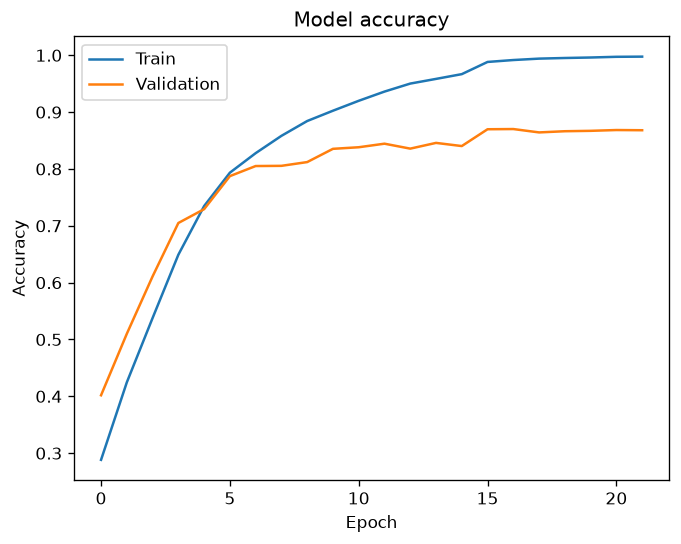
\includegraphics[width=\textwidth]{clasif_VGG_v2_resume_acc.png}
    \caption{Exactitud}
  \end{subfigure}\hfill
  \begin{subfigure}{0.48\textwidth}
    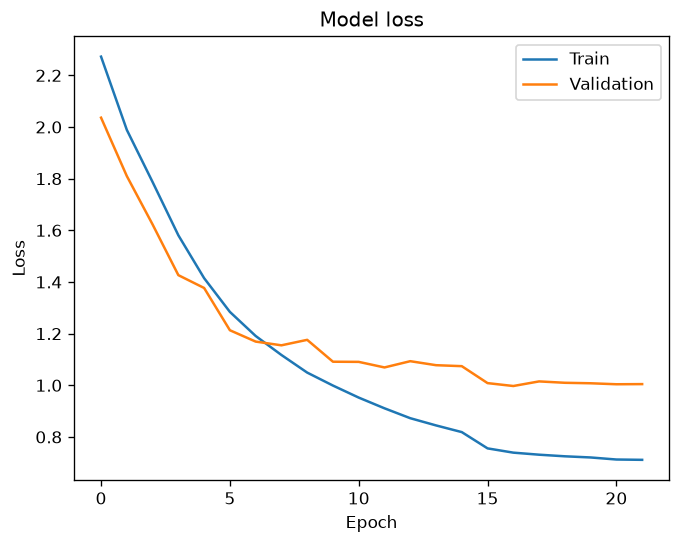
\includegraphics[width=\textwidth]{clasif_VGG_v2_resume_loss.png}
    \caption{Pérdida}
  \end{subfigure}
  \caption{Curvas de entrenamiento y validación del clasificador final (VGG16 + SE +
  \texttt{class\_weight} + \textit{label smoothing} + \(L_2\)).}
  \label{fig:clasif-curvas}
\end{figure}

\subsection{Cariograma}

\pendiente{ejemplo de cariograma ensamblado a partir de una imagen de test.}

\subsection{Interfaz}

La interfaz ejecuta de punta a punta las etapas de pre-procesamiento, segmentación
y extracción/registración, y visualiza cada resultado intermedio
(Figura~\ref{fig:interfaz}). La segmentación corre sobre CPU en pocos segundos
gracias al modelo exportado a TorchScript.

% ================================================================== %
\section{Conclusiones}
\label{sec:conclusiones}
% ================================================================== %

Se desarrolló un pipeline de cariotipado automático que integra pre-procesamiento
caracterizado cuantitativamente, segmentación de instancias con Mask R-CNN,
extracción de características con registración por PCA, clasificación de cada
cromosoma y ensamblado del cariograma, todo accesible desde una interfaz gráfica que
visualiza el procesamiento paso a paso.

\paragraph{Comparación con el estado del arte.} La segmentación desarrollada
(\SI{97.8}{\percent} de AP@0.5) es competitiva con la de Wang \textit{et
al.}~\cite{wang2024fully} (módulo \textit{ChrRender},
\SI{96.65}{\percent}--\SI{96.81}{\percent}) e incluso ligeramente superior, según se
resume en la Tabla~\ref{tab:comparacion}. Debe notarse que aquí se resuelve la
segmentación de una única clase (cromosoma), mientras que parte de la dificultad del
estado del arte proviene de escenarios adicionales; aun así, el resultado ubica a la
etapa de segmentación en un nivel de estado del arte. En clasificación, el modelo
final alcanza un 87\,\% de exactitud, por debajo del \SI{94}{\percent}--\SI{95}{\percent}
del módulo ChrNet4 de Wang \textit{et al.}~\cite{wang2024fully}. La diferencia es
esperable: el modelo del estado del arte incorpora aumentación de datos y un diseño
específico para el problema, mientras que el clasificador aquí desarrollado se
entrenó sin \textit{data augmentation} y sobre un conjunto con marcado desbalance de
clases; el margen de mejora se concentra en los cromosomas de tamaño similar y en la
clase minoritaria.

\begin{table}[H]
  \centering
  \small
  \caption{Comparación con el estado del arte~\cite{wang2024fully}.}
  \label{tab:comparacion}
  \begin{tabular}{lcc}
    \toprule
    & Segmentación (AP@0.5) & Clasificación (exactitud) \\
    \midrule
    Wang \textit{et al.}~\cite{wang2024fully} & 96.7--96.8 & 94--95 \\
    Este trabajo & \textbf{97.8} & 87 \\
    \bottomrule
  \end{tabular}
\end{table}

\paragraph{Posibles mejoras.} Se identifican las siguientes líneas de trabajo:
\begin{itemize}[topsep=2pt,itemsep=1pt]
  \item \textbf{Estudio de ablación} del pre-procesamiento sobre la segmentación,
        confirmando cuantitativamente su robustez a la variación de la entrada.
  \item \textbf{Mejorar la clasificación} incorporando \textit{data augmentation} y
        más muestras de las clases minoritarias, que concentran el error residual.
  \item \textbf{Marcado automático de anomalías numéricas} en el cariograma (por
        ejemplo, un número de instancias por clase distinto de dos).
  \item \textbf{Unificar el entorno de ejecución}: la segmentación usa PyTorch y la
        clasificación TensorFlow; reexportar el clasificador simplificaría el
        despliegue.
\end{itemize}

En síntesis, el trabajo integra un flujo automático de cariotipado con una
segmentación de nivel de estado del arte, una registración que estandariza los
cromosomas y un clasificador que alcanza un 87\,\% de exactitud, y aporta una
interfaz que hace tangible cada etapa del procesamiento de imágenes involucrado.

% ================================================================== %
\appendix
\section{Anexo: detalle de la clasificación}
\label{anexo:clasif}
% ================================================================== %

La Tabla~\ref{tab:clasif-report} presenta el reporte de clasificación por clase del
modelo final. Las Figuras~\ref{fig:anexo-resnet}--\ref{fig:anexo-sev2} muestran las
curvas de entrenamiento del resto de los modelos comparados.

\begin{table}[H]
  \centering
  \small
  \caption{Reporte de clasificación por cromosoma del modelo final (VGG16 + SE +
  \texttt{class\_weight} + \textit{label smoothing} + \(L_2\)). Las clases 23 y 24
  del dataset corresponden a los cromosomas sexuales X e Y, respectivamente.}
  \label{tab:clasif-report}
  \begin{tabular}{lcccc}
    \toprule
    Cromosoma & Precisión & Recall & F1 & Soporte \\
    \midrule
    1  & 0.98 & 0.98 & 0.98 & 132 \\
    2  & 0.95 & 0.95 & 0.95 & 128 \\
    3  & 0.98 & 0.90 & 0.94 & 127 \\
    4  & 0.86 & 0.85 & 0.86 & 126 \\
    5  & 0.90 & 0.91 & 0.90 & 124 \\
    6  & 0.90 & 0.86 & 0.88 & 127 \\
    7  & 0.99 & 0.87 & 0.93 & 128 \\
    8  & 0.85 & 0.90 & 0.87 & 122 \\
    9  & 0.86 & 0.82 & 0.84 & 129 \\
    10 & 0.81 & 0.89 & 0.85 & 129 \\
    11 & 0.91 & 0.94 & 0.92 & 128 \\
    12 & 0.97 & 0.94 & 0.95 & 126 \\
    13 & 0.92 & 0.88 & 0.90 & 122 \\
    14 & 0.91 & 0.87 & 0.89 & 121 \\
    15 & 0.83 & 0.87 & 0.85 & 126 \\
    16 & 0.84 & 0.83 & 0.84 & 125 \\
    17 & 0.82 & 0.78 & 0.80 & 125 \\
    18 & 0.84 & 0.77 & 0.81 & 119 \\
    19 & 0.71 & 0.75 & 0.73 & 116 \\
    20 & 0.73 & 0.87 & 0.80 & 123 \\
    21 & 0.92 & 0.92 & 0.92 & 124 \\
    22 & 0.78 & 0.83 & 0.81 & 123 \\
    X (23) & 0.81 & 0.83 & 0.82 & 100 \\
    Y (24) & 0.68 & 0.71 & 0.69 & 24 \\
    \midrule
    \textbf{Exactitud}        & \multicolumn{3}{c}{\textbf{0.87}} & 2874 \\
    \textit{Promedio macro}   & 0.87 & 0.86 & 0.86 & 2874 \\
    \textit{Promedio ponder.} & 0.87 & 0.87 & 0.87 & 2874 \\
    \bottomrule
  \end{tabular}
\end{table}

\begin{figure}[H]
  \centering
  \begin{subfigure}{0.48\textwidth}
    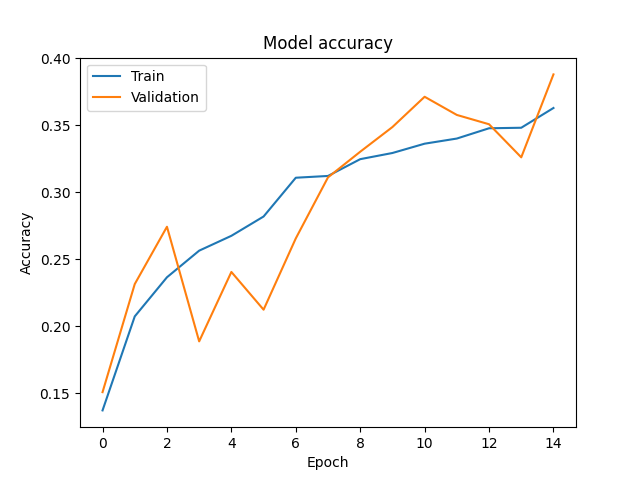
\includegraphics[width=\textwidth]{AccuracyEvolResNet50.png}
    \caption{Exactitud}
  \end{subfigure}\hfill
  \begin{subfigure}{0.48\textwidth}
    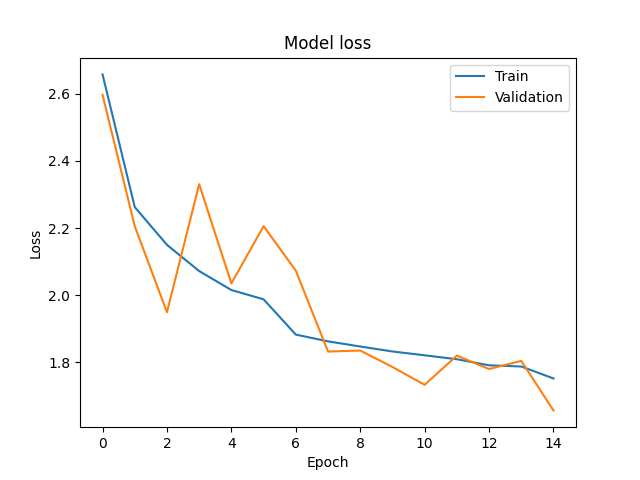
\includegraphics[width=\textwidth]{LossEvolResNet50.png}
    \caption{Pérdida}
  \end{subfigure}
  \caption{ResNet-50: curvas de entrenamiento y validación.}
  \label{fig:anexo-resnet}
\end{figure}

\begin{figure}[H]
  \centering
  \begin{subfigure}{0.48\textwidth}
    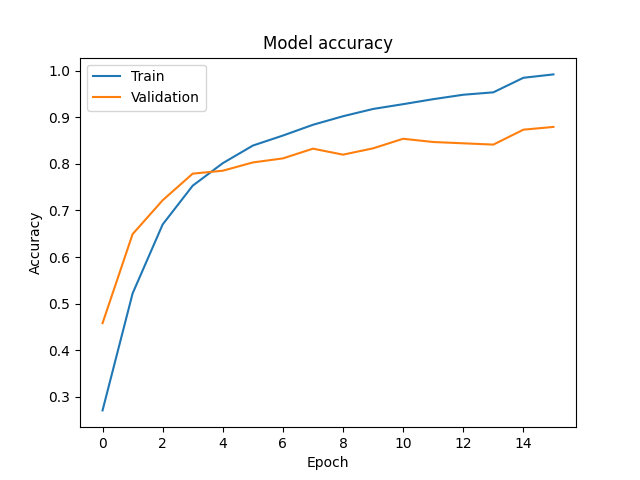
\includegraphics[width=\textwidth]{AccuracyVGG.png}
    \caption{Exactitud}
  \end{subfigure}\hfill
  \begin{subfigure}{0.48\textwidth}
    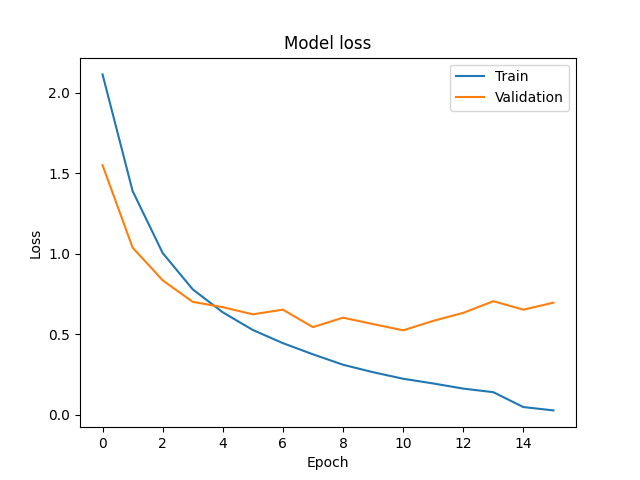
\includegraphics[width=\textwidth]{LossVGG.png}
    \caption{Pérdida}
  \end{subfigure}
  \caption{VGG16 (baseline): curvas de entrenamiento y validación.}
  \label{fig:anexo-vggbase}
\end{figure}

\begin{figure}[H]
  \centering
  \begin{subfigure}{0.48\textwidth}
    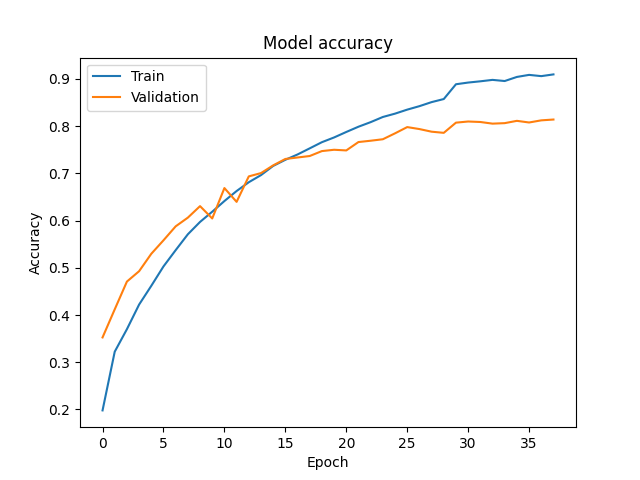
\includegraphics[width=\textwidth]{AtVGGAcc.png}
    \caption{Exactitud}
  \end{subfigure}\hfill
  \begin{subfigure}{0.48\textwidth}
    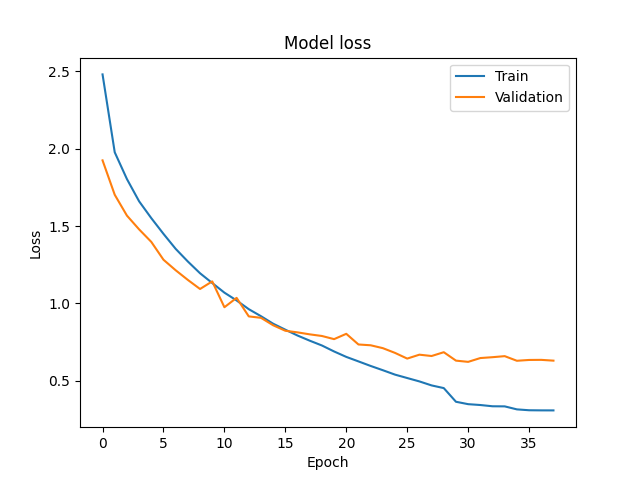
\includegraphics[width=\textwidth]{AtVGGLoss.png}
    \caption{Pérdida}
  \end{subfigure}
  \caption{VGG16 + SE v1: curvas de entrenamiento y validación.}
  \label{fig:anexo-sev1}
\end{figure}

\begin{figure}[H]
  \centering
  \begin{subfigure}{0.48\textwidth}
    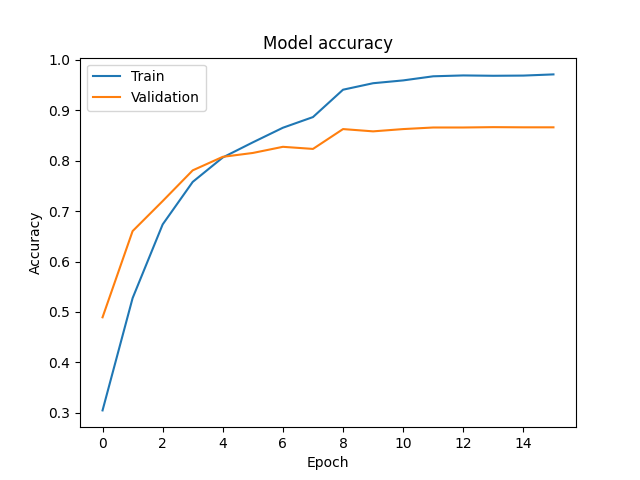
\includegraphics[width=\textwidth]{VGGAt2Acc.png}
    \caption{Exactitud}
  \end{subfigure}\hfill
  \begin{subfigure}{0.48\textwidth}
    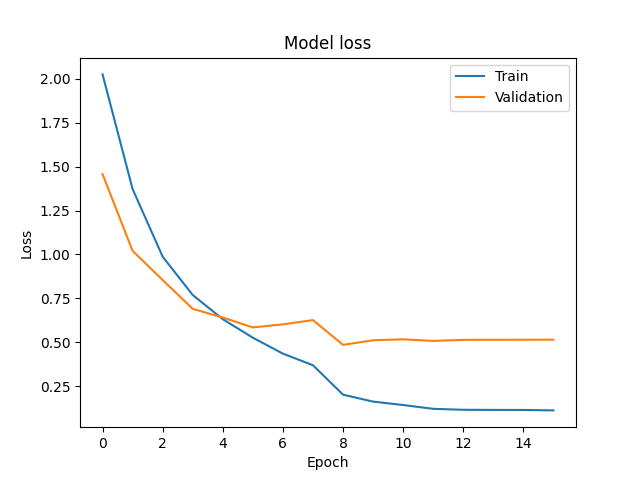
\includegraphics[width=\textwidth]{VGGAt2Loss.png}
    \caption{Pérdida}
  \end{subfigure}
  \caption{VGG16 + SE v2: curvas de entrenamiento y validación.}
  \label{fig:anexo-sev2}
\end{figure}

\bibliographystyle{IEEEtran}
\bibliography{referencias}

\end{document}
